\documentclass[11pt,a4paper]{article}
\usepackage{fontspec}
\usepackage{xeCJK}
\setCJKmainfont{STSong}
\setCJKsansfont{STHeiti}
\usepackage{amsmath,amssymb}
\usepackage{mathtools}
\usepackage{bm}
\usepackage{booktabs}
\usepackage{array}
\usepackage{geometry}
\usepackage{xcolor}
\usepackage{tcolorbox}
\usepackage{tikz}
\usetikzlibrary{arrows.meta,positioning,calc,fit,shapes.geometric}
\usepackage[pdfencoding=auto,psdextra]{hyperref}

\geometry{margin=2.5cm}

\newcommand{\softmax}{\mathrm{softmax}}
\newcommand{\concat}{\mathbin\Vert}
\newcommand{\R}{\mathbb{R}}

\title{\textbf{MoF 路由网络架构数据流分析}\\[0.3em]
\large LUT · adaLN Router · MLP Router}
\author{Flow Factory}
\date{}

\begin{document}
\maketitle

% ═══════════════════════════════════════════════════════════════════
\section{概述}
% ═══════════════════════════════════════════════════════════════════

MoF (Mixture-of-Flow) 使用一个\textbf{路由模块}来预测每个 denoising step 中各 teacher 的混合权重。系统实现了五种路由架构，共享相同的外部接口：

\begin{center}
\begin{tabular}{lll}
\toprule
\textbf{架构} & \textbf{配置名} & \textbf{核心思想} \\
\midrule
离散查找表 (LUT) & \texttt{lut} & 固定 $(K, T, S)$ 参数，按 source × timestep 查表 \\
源无关 LUT (LUT-SA) & \texttt{lut\_simple} & 固定 $(K, T)$ 参数，仅按 timestep 查表 \\
时间路由器 (Time Router) & \texttt{time\_router} & 连续 $t \to W$ 的小型 MLP，无文本输入 \\
adaLN Router & \texttt{adaln\_router} & 时间调制文本，类 DiT 的 adaLN 模式 \\
MLP Router & \texttt{mlp\_router} & 拼接时间+文本，简单 MLP 预测 \\
\bottomrule
\end{tabular}
\end{center}

\textbf{统一输出}：所有架构输出 $\mathbf{W} \in \R^{K \times B}$，其中 $K$ = teacher 数量，$B$ = batch size，每列归一化 $\sum_k W_{k,b} = 1$。

% ═══════════════════════════════════════════════════════════════════
\section{架构 1：离散查找表 (MoFMixingModule)}
% ═══════════════════════════════════════════════════════════════════

\subsection{数据流图}

\begin{center}
\begin{tikzpicture}[
    box/.style={draw, rounded corners, minimum width=2.8cm, minimum height=0.8cm, align=center, fill=blue!8},
    param/.style={draw, rounded corners, minimum width=2.5cm, minimum height=0.8cm, align=center, fill=orange!15},
    io/.style={draw, rounded corners, minimum width=2.5cm, minimum height=0.8cm, align=center, fill=green!10},
    arr/.style={-{Stealth[length=3mm]}, thick},
]
    % Inputs
    \node[io] (tidx) at (0, 4) {$t_{\text{idx}} \in \mathbb{Z}$\\{\scriptsize timestep index}};
    \node[io] (setids) at (4, 4) {$\mathbf{s} \in \mathbb{Z}^B$\\{\scriptsize set IDs}};

    % Parameter
    \node[param] (logits) at (2, 2.5) {$\bm{\Lambda} \in \R^{K \times T \times S}$\\{\scriptsize learnable logits}};

    % Operations
    \node[box] (index) at (2, 1) {Index: $\bm{\Lambda}[:, t_{\text{idx}}, \mathbf{s}]$};
    \node[box] (softmax) at (2, -0.5) {$\softmax(\cdot / \tau, \text{dim}=0)$};

    % Output
    \node[io] (out) at (2, -2) {$\mathbf{W} \in \R^{K \times B}$\\{\scriptsize 混合权重}};

    % Arrows
    \draw[arr] (tidx) -- (index);
    \draw[arr] (setids) -- (index);
    \draw[arr] (logits) -- (index);
    \draw[arr] (index) -- (softmax);
    \draw[arr] (softmax) -- (out);
\end{tikzpicture}
\end{center}

\subsection{张量维度详解}

\begin{center}
\begin{tabular}{lcp{8cm}}
\toprule
\textbf{张量} & \textbf{形状} & \textbf{维度含义} \\
\midrule
$\bm{\Lambda}$ (logits) & $(K, T, S)$ &
    $K$: teacher 数量 (e.g., 3) \newline
    $T$: denoising 总步数 (e.g., 10) \newline
    $S$: prompt source 集合数 (e.g., 3 for geneval/pickscore/ocr) \\
\midrule
$t_{\text{idx}}$ & scalar $\in [0, T{-}1]$ & 当前 denoising step 的整数索引 \\
\midrule
$\mathbf{s}$ (set\_ids) & $(B,)$ & 每个样本对应的 source 集合 ID \\
\midrule
$\bm{\Lambda}[:, t_{\text{idx}}, :]$ & $(K, S)$ & 当前 step 下所有 teacher × 所有 source 的 logits \\
\midrule
$\bm{\Lambda}[:, t_{\text{idx}}, \mathbf{s}]$ & $(K, B)$ & 每样本取对应 source 的 logits (advanced indexing) \\
\midrule
$\mathbf{W}$ & $(K, B)$ & softmax 归一化后的权重，$\sum_k W_{k,b} = 1$ \\
\bottomrule
\end{tabular}
\end{center}

\subsection{计算逻辑}

\begin{equation}
W_{k,b} = \frac{\exp(\Lambda_{k, t_{\text{idx}}, s_b} / \tau)}{\sum_{k'=1}^K \exp(\Lambda_{k', t_{\text{idx}}, s_b} / \tau)}
\end{equation}

\textbf{特点}：无神经网络计算，纯查表 + softmax。$K \times T \times S$ 个可学习参数。

% ═══════════════════════════════════════════════════════════════════
\section{架构 1B：源无关 LUT (MoFMixingModuleSimple, ``LUT-SA'')}
\label{sec:lut_sa}
% ═══════════════════════════════════════════════════════════════════

\subsection{动机}

源无关 LUT (\texttt{lut\_simple}) 是源感知 LUT 的简化版本：丢弃 $S$ 轴，只保留 $(K, T)$ 两个维度。

\begin{tcolorbox}[colback=blue!5, colframe=blue!50, title=核心问题]
\textbf{若不同 source 的最优 teacher 混合相似，是否仍需要为每个 source 单独学一组 logits？}
\end{tcolorbox}

LUT-SA 用一个共享的 $(K, T)$ 表回答这个问题：所有样本共享同一套 per-timestep 权重，但 \textbf{reward / advantage 仍然按 source 路由}（$A_b = a_{\text{in}}(s_b) + \gamma \cdot \text{mean}(a_{\text{ood}})$）。这给出了一个干净的对照实验：若 LUT-SA 与 LUT 性能持平，说明 per-source 维度对当前问题冗余；若 LUT 显著更好，说明 teacher 间存在需要按 source 区分的专长边界。

\subsection{数据流图}

\begin{center}
\begin{tikzpicture}[
    box/.style={draw, rounded corners, minimum width=2.8cm, minimum height=0.8cm, align=center, fill=blue!8},
    param/.style={draw, rounded corners, minimum width=2.5cm, minimum height=0.8cm, align=center, fill=orange!15},
    io/.style={draw, rounded corners, minimum width=2.5cm, minimum height=0.8cm, align=center, fill=green!10},
    arr/.style={-{Stealth[length=3mm]}, thick},
]
    % Inputs
    \node[io] (tidx) at (0, 4) {$t_{\text{idx}} \in \mathbb{Z}$\\{\scriptsize timestep index}};

    % Parameter
    \node[param] (logits) at (0, 2.5) {$\bm{\Lambda} \in \R^{K \times T}$\\{\scriptsize learnable logits, no $S$}};

    % Operations
    \node[box] (index) at (0, 1) {Index: $\bm{\Lambda}[:, t_{\text{idx}}]$};
    \node[box] (softmax) at (0, -0.5) {$\softmax(\cdot / \tau, \text{dim}=0)$};
    \node[box, fill=yellow!15] (broad) at (0, -2) {Broadcast over $B$\\{\scriptsize $(K) \to (K, B)$}};

    % Output
    \node[io] (out) at (0, -3.5) {$\mathbf{W} \in \R^{K \times B}$\\{\scriptsize 所有列相同}};

    % Arrows
    \draw[arr] (tidx) -- (index);
    \draw[arr] (logits) -- (index);
    \draw[arr] (index) -- (softmax);
    \draw[arr] (softmax) -- (broad);
    \draw[arr] (broad) -- (out);
\end{tikzpicture}
\end{center}

\subsection{计算逻辑}

\begin{align}
W_{k,b} = W_k(t_{\text{idx}}) &= \frac{\exp(\Lambda_{k, t_{\text{idx}}} / \tau)}{\sum_{k'=1}^K \exp(\Lambda_{k', t_{\text{idx}}} / \tau)}, \quad \forall b \in [1, B]
\label{eq:lut_sa_weight}
\end{align}

注意右侧不依赖 $b$（也不依赖 $s_b$、$\mathbf{c}_b$），所以 $\mathbf{W}$ 在 batch 内沿 $B$ 轴常数广播。

\subsection{API 兼容性：广播到 $(K, T, S)$}

为了让下游代码（按 \texttt{set\_ids} 高级索引）无需任何修改，\texttt{forward()} 输出形状仍为 $(K, T, S)$，但所有 $S$ 切片相等：

\begin{equation}
\mathbf{W}_{\text{out}}[k, t, s] = W_k(t), \quad \forall s \in [0, S{-}1]
\end{equation}

这是一个零成本的 \texttt{expand} 视图（不复制内存），参数仍只有 $K \cdot T$ 个。

\subsection{优化目标与梯度流}

考虑学生在第 $b$ 个样本上的 NFT/GRPO 损失，其优势 $A_b = A(x_b, s_b)$ 由 source-aware 的 advantage pipeline（in-domain + $\gamma \cdot$ mean(ood)）给出。logits $\bm{\Lambda}$ 的梯度为：

\begin{equation}
\nabla_{\Lambda_{k,t}} \mathcal{L}
= \mathbb{E}_{(x, s) \sim \mathcal{D}} \left[
    A(x, s) \cdot \nabla_{\Lambda_{k,t}} \log p_\theta(x \mid t)
\right]
\label{eq:lut_sa_grad}
\end{equation}

由于 $\Lambda_{k,t}$ 不依赖 $s$，所有 source 的样本梯度都流入\textbf{同一个} $\Lambda_{k,t}$ 参数。最优解满足：

\begin{equation}
\Lambda^*(:, t) = \arg\max_{\Lambda(:, t)} \;
\mathbb{E}_{s \sim P(s)} \mathbb{E}_{x \sim p_\Lambda(\cdot \mid s, t)}
\bigl[ R_s(x) + \gamma \cdot \tfrac{1}{|J|}\textstyle\sum_{j \in J} R_j(x) \bigr]
\label{eq:lut_sa_optimal}
\end{equation}

其中 $J = \{j : j \neq R_{\text{in}}(s)\}$ 为 OOD reward 集合，$P(s)$ 为训练时 source 的边际分布。换言之，LUT-SA 学到的是\textbf{对 source 边际化}（marginalized over $s$）后的最优混合策略。

\subsection{与源感知 LUT 的关系}

LUT-SA 是源感知 LUT 在等约束 $\Lambda_{k,t,1} = \Lambda_{k,t,2} = \cdots = \Lambda_{k,t,S}$ 下的特殊解。从假设空间角度：

\begin{equation}
\mathcal{H}_{\text{LUT-SA}} \subsetneq \mathcal{H}_{\text{LUT}}
\end{equation}

\begin{itemize}
    \item \textbf{LUT 能表达的，LUT-SA 不一定能}：当不同 source 的最优 teacher 混合差异显著时（例如 OCR 偏好 teacher-ocr，GenEval 偏好 teacher-geneval），LUT-SA 必须做妥协。
    \item \textbf{LUT-SA 能表达的，LUT 总能精确复现}：将 LUT 的所有 $S$ 切片设为相等即可。
\end{itemize}

因此 LUT-SA 与 LUT 的性能差距，定量衡量了\textbf{per-source 路由收益}。

\subsection{何时使用 LUT-SA}

\begin{center}
\small
\begin{tabular}{p{4.2cm}|p{4.2cm}|p{4.2cm}}
\toprule
\textbf{推荐使用} & \textbf{中性} & \textbf{不推荐} \\
\midrule
Teacher 互补但不专业化（如多个 LoRA 共享一个底座、风格相近）&
$K = 2$ 时（$S$ 维收益本就不明显）&
Teacher 与 source 严格一一对应（hard-route 配置） \\
\midrule
作为 ablation baseline，定量评估 per-source 路由收益 &
样本量 $N$ 较小时，参数减少有助于防止过拟合 &
不同 source 间 reward scale 差异大且 $\gamma$ 较小 \\
\midrule
推理时希望 source 标签解耦（同 prompt 不同 source 标签得到相同输出）&
& OOD 比例极小（$\gamma \to 0$ 时几乎退化为单 source 训练） \\
\bottomrule
\end{tabular}
\end{center}

\subsection{参数量对比}

\begin{center}
\small
\begin{tabular}{l|cc|c}
\toprule
\textbf{模块} & \textbf{形状} & \textbf{参数量}（$K{=}3, T{=}10, S{=}3$） & \textbf{vs LUT} \\
\midrule
LUT (\texttt{lut}) & $(K, T, S)$ & $90$ & $1.0\times$ \\
\textbf{LUT-SA (\texttt{lut\_simple})} & $\mathbf{(K, T)}$ & $\mathbf{30}$ & $\mathbf{1/S \times}$ \\
adaLN Router & 神经网络 & $\sim 790$K & $\sim 8800\times$ \\
MLP Router & 神经网络 & $\sim 660$K & $\sim 7300\times$ \\
\bottomrule
\end{tabular}
\end{center}

参数量随 $S$ 线性下降。当 $S$ 较大（例如 $S = 10$ 个 source 子集）时，LUT-SA 的参数节省更显著。

\subsection{与 reward 路由的协同}

\textbf{关键不变量}：mixing 模块源无关 $\not\Rightarrow$ reward 源无关。MoF 框架下二者解耦：

\begin{center}
\begin{tabular}{l|c|c}
\toprule
\textbf{机制} & \textbf{Mixing weights} & \textbf{Reward / Advantage} \\
\midrule
LUT (\texttt{lut}) & 源感知 ($\Lambda_{k,t,s}$) & 源感知 ($A_b = a_{\text{in}}(s_b) + \gamma\,\text{mean}(a_{\text{ood}})$) \\
\textbf{LUT-SA (\texttt{lut\_simple})} & \textbf{源无关 ($\Lambda_{k,t}$)} & \textbf{源感知 (同上)} \\
Router & 隐式源感知（经 $\mathbf{c}_b$） & 源感知 (同上) \\
\bottomrule
\end{tabular}
\end{center}

LUT-SA 训练流程（以 NFT 为例）：

\begin{enumerate}
    \item Sample：student 用当前 $W_k(t) = \softmax_k(\Lambda_{k,t}/\tau)$ 混合 teacher 速度，rollout 整条轨迹。
    \item Reward：每个 reward $R_j$ 在自己的 \texttt{applicable\_sources} 子集上计算。
    \item Advantage：按 \eqref{eq:lut_sa_grad} 中的 $A(x, s)$ 公式计算 source-aware advantage。
    \item Loss：将 source-aware $A_b$ 反传到 source-agnostic $\Lambda$，每个 $\Lambda_{k,t}$ 累积所有 source 的梯度信号。
\end{enumerate}

\subsection{实现要点}

\begin{enumerate}
    \item \textbf{Logits 形状}：模块内部 $\bm{\Lambda} \in \R^{K \times T}$，无 $S$ 轴。
    \item \textbf{Forward 输出广播}：\texttt{forward()} 返回 $(K, T, S)$，由 \texttt{logits.unsqueeze(-1).expand(K,T,S)} 实现（视图，不占额外内存）。
    \item \textbf{初始化}：
        \begin{itemize}
            \item \texttt{uniform}：$\bm{\Lambda} = \mathbf{0}$，softmax 后每个 teacher $1/K$。
            \item \texttt{teacher\_biased}：因无 $S$ 轴可独立偏置，将所有 source 的 in-domain teacher 偏置\emph{合并}到统一的 $\bm{\Lambda}$ 行（多 source 同一 teacher 时偏置叠加）。
        \end{itemize}
    \item \texttt{ema}、checkpoint、distill 加载：与源感知 LUT 共用代码路径；distill 加载时若发现 \texttt{lambda\_logits} 为 2D 张量，会自动 \texttt{unsqueeze(-1).expand} 到 $(K, T, S)$ 后再过 softmax。
\end{enumerate}

% ═══════════════════════════════════════════════════════════════════
\section{架构 1C：时间路由器 (MoFTimeRouter, ``Time Router'')}
\label{sec:time_router}
% ═══════════════════════════════════════════════════════════════════

\subsection{动机：从离散查表到连续时间函数}

LUT-SA 抹掉了 $S$ 轴，但仍保留 $T$ 轴的离散查表结构，这意味着：

\begin{itemize}
    \item 训练与推理必须使用\textbf{相同的} $T$（推理时第 $i$ 步固定查 $\bm{\Lambda}[:, i]$）。
    \item 相邻 timestep 的权重之间无显式连续性约束——网络可以学到任意跳跃的混合曲线。
\end{itemize}

时间路由器进一步把离散查表替换为关于 $t$ 的\textbf{连续函数} $W: \R \to \Delta^{K-1}$，但\textbf{不引入文本条件}：

\begin{tcolorbox}[colback=blue!5, colframe=blue!50, title=核心问题]
若混合策略只随 timestep 平滑变化，与 prompt 内容无关，能否用一个仅以 $t$ 为输入的小型 MLP 替代离散 LUT？这种参数化能否在保持表达力的同时获得\textbf{推理 $T$ 灵活性}？
\end{tcolorbox}

\textbf{设计定位}：Time Router 是连续时间路由器中的最简变体——只有时间分支，没有文本分支。它在假设空间和参数效率上位于 LUT-SA 与全路由器之间：

\begin{center}
\small
\begin{tabular}{l|cccc}
\toprule
\textbf{模块} & \textbf{时间} & \textbf{文本/Source} & \textbf{时间平滑性} & \textbf{推理 $T$} \\
\midrule
LUT          & 离散查表 & source-aware       & 任意（可跳跃）  & 绑定训练 $T$ \\
LUT-SA       & 离散查表 & 无（边际化）       & 任意（可跳跃）  & 绑定训练 $T$ \\
\textbf{Time Router} & \textbf{连续 NN} & \textbf{无} & \textbf{隐式平滑} & \textbf{任意 $T$} \\
adaLN Router & 连续 NN  & 隐式经 prompt      & 隐式平滑        & 任意 $T$ \\
MLP Router   & 连续 NN  & 隐式经 prompt      & 隐式平滑        & 任意 $T$ \\
\bottomrule
\end{tabular}
\end{center}

\subsection{数据流图}

\begin{center}
\begin{tikzpicture}[
    box/.style={draw, rounded corners, minimum width=3cm, minimum height=0.8cm, align=center, fill=blue!8},
    io/.style={draw, rounded corners, minimum width=3cm, minimum height=0.8cm, align=center, fill=green!10},
    arr/.style={-{Stealth[length=3mm]}, thick},
]
    % Input
    \node[io] (t_in) at (0, 5) {$\mathbf{t} \in \R^B$\\{\scriptsize raw timestep}};

    % Time branch (no text branch)
    \node[box] (sinemb) at (0, 3.5) {SinusoidalPosEmb\\{\scriptsize $\R^B \to \R^{B \times d_t}$}};
    \node[box] (lin1) at (0, 2) {Linear$_1$ + SiLU\\{\scriptsize $\R^{B \times d_t} \to \R^{B \times d_h}$}};
    \node[box] (lin2) at (0, 0.5) {Linear$_2$ + SiLU\\{\scriptsize $\R^{B \times d_h} \to \R^{B \times d_h}$}};
    \node[box, fill=red!10] (out_lin) at (0, -1) {Linear$_{\text{out}}$ \emph{(零初始化)}\\{\scriptsize $\R^{B \times d_h} \to \R^{B \times K}$}};
    \node[box] (sm) at (0, -2.5) {$\softmax(\cdot / \tau, \text{dim}{=}{-}1)$};
    \node[io] (out) at (0, -4) {$\mathbf{W} \in \R^{K \times B}$ {\scriptsize (转置)}};

    \draw[arr] (t_in) -- (sinemb);
    \draw[arr] (sinemb) -- (lin1);
    \draw[arr] (lin1) -- (lin2);
    \draw[arr] (lin2) -- (out_lin);
    \draw[arr] (out_lin) -- (sm);
    \draw[arr] (sm) -- (out);
\end{tikzpicture}
\end{center}

\textbf{关键观察}：与 adaLN/MLP Router 相比，Time Router\textbf{完全删除了文本分支}（c\_proj、AttnPool）以及融合层（adaLN 调制或 concat）。前向路径只有时间分支 + 输出分类头。

\subsection{张量维度详解}

\begin{center}
\small
\begin{tabular}{lcp{7.5cm}}
\toprule
\textbf{张量} & \textbf{形状} & \textbf{维度含义} \\
\midrule
\multicolumn{3}{l}{\textit{--- 输入 ---}} \\
$\mathbf{t}$ & $(B,)$ & 每样本的 raw timestep 值（scheduler 原始尺度，e.g. 0--1000） \\
\midrule
\multicolumn{3}{l}{\textit{--- Time Branch ---}} \\
SinusoidalEmb($\mathbf{t}$) & $(B, d_t)$ & 正弦位置编码（$d_t$=256，复用 \texttt{mixing\_d\_time}） \\
$\mathbf{h}_1$ = Linear$_1$+SiLU & $(B, d_h)$ & 第一隐层（$d_h$=256，复用 \texttt{mixing\_hidden\_dim}） \\
$\mathbf{h}_2$ = Linear$_2$+SiLU & $(B, d_h)$ & 第二隐层 \\
\midrule
\multicolumn{3}{l}{\textit{--- 输出 ---}} \\
$\bm{\ell}$ = Linear$_{\text{out}}(\mathbf{h}_2)$ & $(B, K)$ & 未归一化 logits（输出层零初始化 → 起始权重 $1/K$） \\
$\mathbf{W}$ & $(K, B)$ & softmax + transpose，$\sum_k W_{k,b} = 1$ \\
\bottomrule
\end{tabular}
\end{center}

\textbf{注}：Time Router 不使用 \texttt{mixing\_d\_pool} 和 \texttt{mixing\_d\_seq}（无文本路径）。即使 config 中设置了这两个字段，模块也会忽略。

\subsection{计算逻辑}

\begin{align}
\mathbf{e}_t &= \text{SinusoidalPosEmb}_{d_t}(\mathbf{t}) && \in \R^{B \times d_t} \\
\mathbf{h}_1 &= \text{SiLU}(\text{Linear}_1(\mathbf{e}_t)) && \in \R^{B \times d_h} \\
\mathbf{h}_2 &= \text{SiLU}(\text{Linear}_2(\mathbf{h}_1)) && \in \R^{B \times d_h} \\
\bm{\ell} &= \text{Linear}_{\text{out}}(\mathbf{h}_2) && \in \R^{B \times K} \quad \text{(输出层零初始化)} \\
W_{k,b} &= \softmax(\bm{\ell}_b / \tau)_k
\end{align}

\textbf{关键性质}：当 batch 内所有样本共享同一个 $t_b$ 时（典型 MoF 推理与训练 timestep 采样模式），$\mathbf{W}$ 的所有列相等。当 $t_b$ 在 batch 内不同时（少见），网络自然给出 $B$ 个不同的混合向量。

\subsection{优化目标与梯度流}

设训练 timestep 集合为 $\mathcal{T}_{\text{train}} = \{t_0, t_1, \ldots, t_{T-1}\}$。Time Router 的优化目标：

\begin{equation}
\min_{\theta_{\text{TR}}} \mathbb{E}_{(x, s, t) \sim \mathcal{D}} \left[
    -A(x, s) \cdot \log p_{\theta_{\text{TR}}}(x \mid t)
\right]
\label{eq:time_router_obj}
\end{equation}

其中 $\theta_{\text{TR}} = \{\text{Linear}_1, \text{Linear}_2, \text{Linear}_{\text{out}}\}$ 为路由器权重，$p_{\theta_{\text{TR}}}(x|t)$ 表示用 $W_k(t; \theta_{\text{TR}})$ 混合 teacher 速度后的学生轨迹密度。

由于 $W$ 完全由 $\theta_{\text{TR}}$ 控制（不依赖 $s$），所有 source 的样本梯度通过\textbf{同一组共享权重}流动：

\begin{equation}
\nabla_{\theta_{\text{TR}}} \mathcal{L}
= \mathbb{E}_{(x, s, t)} \left[
    A(x, s) \cdot \sum_{k=1}^K \frac{\partial \log p}{\partial W_k(t)} \cdot \nabla_{\theta_{\text{TR}}} W_k(t)
\right]
\label{eq:time_router_grad}
\end{equation}

注意 $\nabla_{\theta_{\text{TR}}} W_k(t)$ 只依赖 $t$——这表明 Time Router 的所有参数更新对所有 $t$ 同时生效（与 LUT-SA 中 $\Lambda(:,t)$ 仅由对应 timestep 的样本更新形成对照）。

\subsection{假设空间分析}

\subsubsection{在训练 timestep 上的等价性}

形式上，Time Router 限制在训练 timestep 集合 $\mathcal{T}_{\text{train}}$ 上的输出空间满足：

\begin{equation}
\mathcal{H}_{\text{TR}}\big|_{\mathcal{T}_{\text{train}}} \subseteq \mathcal{H}_{\text{LUT-SA}}
\label{eq:tr_subset_lut}
\end{equation}

LUT-SA 在 $\mathcal{T}_{\text{train}}$ 上有 $K \cdot T$ 个独立自由度；Time Router 受 NN 参数化约束，等效自由度更低（任何相邻 $t_i$ 的输出都通过共享权重耦合）。

\subsubsection{在连续时间上的扩展性}

但在 $\mathcal{T}_{\text{train}}$ 之外（连续 $t \in \R$）：

\begin{equation}
\mathcal{H}_{\text{TR}}\big|_{\R} \not\subseteq \mathcal{H}_{\text{LUT-SA}}
\end{equation}

LUT-SA 在 $\mathcal{T}_{\text{train}}$ 之外\textbf{完全没有定义}——它无法回答"$t = 0.5(t_3 + t_4)$ 时的混合权重应该是多少"。Time Router 通过 NN 自然外推：

\begin{equation}
W_{\text{TR}}(t^*) = \softmax\bigl(\text{MLP}_\theta(\text{SinusoidalEmb}(t^*)) / \tau\bigr), \quad \forall t^* \in \R
\end{equation}

这给了 Time Router 一个独有的优势：\textbf{推理时可以使用任意数量的 timestep}（即使训练时只用了 $T=10$，推理可以用 $T=20$ 或 $T=50$，无需重训）。

\subsubsection{平滑性的归纳偏置}

由于 NN 的 Lipschitz 连续性（线性层 + SiLU 激活），Time Router 隐式地对 $W(t)$ 施加平滑性约束。这是一把双刃剑：

\begin{center}
\begin{tabular}{p{6cm}|p{6cm}}
\toprule
\textbf{平滑性的好处} & \textbf{平滑性的代价} \\
\midrule
若最优混合策略本就随 $t$ 平滑变化（典型情况），NN 的归纳偏置作为\emph{隐式正则化}，在 RL 信号稀疏时（每 epoch 144 样本）抑制过拟合。 &
若最优策略在某些 $t$ 处需要尖锐切换（e.g. 高 noise 区与低 noise 区使用完全不同的 teacher 集合），平滑 NN 在切换点附近的表达受限。 \\
\midrule
SinusoidalEmb 的多频率分量允许网络在需要时学到中等频率的振荡，缓解上述问题。 &
极端的不连续（阶跃函数）仍难以精确刻画。
\\
\bottomrule
\end{tabular}
\end{center}

\subsection{何时使用 Time Router}

\begin{center}
\small
\begin{tabular}{p{4.2cm}|p{4.2cm}|p{4.2cm}}
\toprule
\textbf{推荐使用} & \textbf{中性} & \textbf{不推荐} \\
\midrule
推理需要灵活的 timestep 数量（训练 $T_{\text{train}}$，推理 $T_{\text{infer}} \neq T_{\text{train}}$） &
RL 训练样本稀疏，需要平滑性正则化 &
最优混合策略需要按 prompt 内容路由（e.g. teacher\_geneval 仅适用于含计数/物体的 prompt） \\
\midrule
作为\emph{简化对照}测试 prompt 路由必要性：若与 adaLN/MLP Router 性能持平，说明 prompt 不影响路由决策 &
$K$ 较大（5--10）时，连续参数化能在不大幅增加参数下提升表达力 &
最优策略在某些 $t$ 处有尖锐切换且训练 $T$ 足够密集（LUT-SA 此时更直接） \\
\midrule
模型部署时不希望路由器依赖文本编码器输出（解耦推理 pipeline） & & 训练数据极少（平滑 NN 的 132K 参数仍可能过拟合） \\
\bottomrule
\end{tabular}
\end{center}

\subsection{参数量对比}

\begin{center}
\small
\begin{tabular}{l|cc|c|c}
\toprule
\textbf{模块} & \textbf{形状} & \textbf{参数量}（K=3, T=10, S=3, $d_h$=256, $d_t$=256） & \textbf{vs LUT} & \textbf{vs adaLN} \\
\midrule
LUT (\texttt{lut}) & $(K, T, S)$ logits & $90$ & $1.0\times$ & $\sim 1/8800\times$ \\
LUT-SA (\texttt{lut\_simple}) & $(K, T)$ logits & $30$ & $1/3 \times$ & $\sim 1/26000\times$ \\
\textbf{Time Router} (\texttt{time\_router}) & 3 Linear & $\mathbf{\sim 132K}$ & $\sim 1500\times$ & $\sim 1/6 \times$ \\
adaLN Router & adaLN + 2 branches & $\sim 790$K & $\sim 8800\times$ & $1.0\times$ \\
MLP Router & concat + 3 Linear & $\sim 660$K & $\sim 7300\times$ & $\sim 5/6 \times$ \\
\bottomrule
\end{tabular}
\end{center}

具体计算（$K=3$, $d_t = d_h = 256$）：
\begin{align}
\text{Linear}_1: & \quad 256 \times 256 + 256 = 65{,}792 \\
\text{Linear}_2: & \quad 256 \times 256 + 256 = 65{,}792 \\
\text{Linear}_{\text{out}}: & \quad 256 \times 3 + 3 = 771 \\
\text{Total}: & \quad 132{,}355 \approx 132\text{K}
\end{align}

参数节省主要来自删除了 c\_proj（$2048 \times 256 \approx 525$K params）和 AttnPool（如使用，约 $4096 \times 256 \approx 1$M params）。

\subsection{与 reward 路由的协同}

\textbf{关键不变量}：与 LUT-SA 一样，mixing 模块的源无关性\textbf{不影响} reward / advantage 的源感知性。三种"源无关 mixing + 源感知 reward"的组合：

\begin{center}
\begin{tabular}{l|c|c|c}
\toprule
\textbf{机制} & \textbf{Mixing 输入} & \textbf{时间 sharpness} & \textbf{推理 $T$} \\
\midrule
LUT-SA (\texttt{lut\_simple}) & 仅 $t$ (整数索引) & 任意 & 绑定训练 $T$ \\
\textbf{Time Router (\texttt{time\_router})} & \textbf{仅 $t$ (连续)} & \textbf{隐式平滑} & \textbf{任意 $T$} \\
adaLN/MLP Router & $t$ + prompt content & 隐式平滑 & 任意 $T$ \\
\bottomrule
\end{tabular}
\end{center}

不论选哪一种 mixing 模块，advantage 计算路径完全相同：

\begin{equation}
A(x_b, s_b) = a_{R_{\text{in}}(s_b)}(x_b) + \gamma \cdot \tfrac{1}{|J|}\textstyle\sum_{j \in J} a_j(x_b)
\end{equation}

Time Router 的训练流程：

\begin{enumerate}
    \item Sample：student 用当前 $W_k(t; \theta_{\text{TR}})$ 混合 teacher 速度，rollout 整条轨迹。
    \item Reward：每个 reward 在自己的 \texttt{applicable\_sources} 子集上计算。
    \item Advantage：按 source-aware 的 in-domain + γ·OOD 公式计算 $A_b$。
    \item Loss：source-aware $A_b$ 反传到 source-agnostic $\theta_{\text{TR}}$，所有 timestep 的样本共享对路由器权重的更新。
\end{enumerate}

\subsection{实现要点}

\begin{enumerate}
    \item \textbf{类继承结构}：建议\textbf{不}继承自 \texttt{MoFRouterBase}，因为后者在 \texttt{\_\_init\_\_} 中强制构建 c\_proj（依赖 $d_{\text{pool}}$），会引入对 Time Router 不必要的字段依赖。直接继承 \texttt{nn.Module}，自包含 SinusoidalPosEmb + 时间 MLP + 输出头即可。
    \item \textbf{Forward 签名兼容}：为与现有路由器调用点兼容，签名可设计为 \texttt{forward(t, prompt\_embeds=None, pooled\_prompt\_embeds=None)} 但忽略后两个参数。这样 \texttt{patched\_forward} 中的 \texttt{w\_i = router(t, prompt\_emb, pooled)} 调用无需修改。
    \item \textbf{零初始化}：\texttt{Linear}$_{\text{out}}$ 的 weight 和 bias 都初始化为零 → 训练初期所有 teacher 均匀加权 $1/K$。这与 adaLN/MLP Router 的零初始化策略一致。
    \item \textbf{无需文本配置}：模块创建时只读取 \texttt{mixing\_d\_time}（默认 256）和 \texttt{mixing\_hidden\_dim}（默认 256）；忽略 \texttt{mixing\_d\_pool} 和 \texttt{mixing\_d\_seq}。
    \item \textbf{Checkpoint 元数据}：\texttt{router\_arch} 字典中 \texttt{d\_pool=None}, \texttt{d\_seq=None}, 其余字段（\texttt{K}, \texttt{d\_hidden}, \texttt{d\_time}, \texttt{tau}）正常填写。Distill 加载时识别出 \texttt{d\_pool=None} 即可重建 Time Router。
    \item \textbf{推理时 timestep 灵活性}：$\texttt{num\_inference\_steps}$ 在训练和推理可不一致；调度器在推理时间用任何 $T_{\text{infer}}$ 离散化连续时间区间，把每个采样到的 $t$ 喂给 Time Router 即可获得对应混合权重。
\end{enumerate}

% ═══════════════════════════════════════════════════════════════════
\section{架构 2：adaLN Router (MoFAdaLNRouter)}
% ═══════════════════════════════════════════════════════════════════

\subsection{数据流图}

\begin{center}
\begin{tikzpicture}[
    box/.style={draw, rounded corners, minimum width=3cm, minimum height=0.8cm, align=center, fill=blue!8},
    param/.style={draw, rounded corners, minimum width=2.5cm, minimum height=0.8cm, align=center, fill=orange!15},
    io/.style={draw, rounded corners, minimum width=3cm, minimum height=0.8cm, align=center, fill=green!10},
    arr/.style={-{Stealth[length=3mm]}, thick},
    node distance=0.8cm,
]
    % Inputs
    \node[io] (t_in) at (-3, 6) {$\mathbf{t} \in \R^B$\\{\scriptsize raw timestep}};
    \node[io] (pe_in) at (3, 6) {$\mathbf{H} \in \R^{B \times L \times d_{\text{text}}}$\\{\scriptsize prompt\_embeds}};

    % Time branch
    \node[box] (sinemb) at (-3, 4.5) {SinusoidalEmb\\{\scriptsize $\R^B \to \R^{B \times d_t}$}};
    \node[box] (tmlp) at (-3, 3) {Linear + SiLU\\{\scriptsize $\R^{B \times d_t} \to \R^{B \times d_h}$}};
    \node[box] (adaln) at (-3, 1.5) {Linear (adaLN)\\{\scriptsize $\R^{B \times d_h} \to \R^{B \times 2d_h}$}};
    \node[box] (chunk) at (-3, 0) {chunk $\to (\gamma, \beta)$\\{\scriptsize 各 $\R^{B \times d_h}$}};

    % Text branch
    \node[box] (attnpool) at (3, 4.5) {AttnPool($\mathbf{q}$)\\{\scriptsize $\R^{B \times L \times d_{\text{text}}} \to \R^{B \times d_{\text{text}}}$}};
    \node[box] (cproj) at (3, 3) {Linear (c\_proj)\\{\scriptsize $\R^{B \times d_{\text{text}}} \to \R^{B \times d_h}$}};

    % Fusion
    \node[box, fill=red!10, minimum width=4cm] (fuse) at (0, -1.5) {$\mathbf{h} = \gamma \odot \mathbf{c} + \beta$\\{\scriptsize adaLN modulation, $\R^{B \times d_h}$}};

    % Output MLP
    \node[box] (mlp) at (0, -3) {SiLU → Linear → SiLU → Linear\\{\scriptsize $\R^{B \times d_h} \to \R^{B \times K}$}};
    \node[box] (sm) at (0, -4.5) {$\softmax(\cdot / \tau, \text{dim}{=}{-}1)$};
    \node[io] (out) at (0, -6) {$\mathbf{W} \in \R^{K \times B}$ {\scriptsize (transposed)}};

    % Arrows
    \draw[arr] (t_in) -- (sinemb);
    \draw[arr] (sinemb) -- (tmlp);
    \draw[arr] (tmlp) -- (adaln);
    \draw[arr] (adaln) -- (chunk);
    \draw[arr] (pe_in) -- (attnpool);
    \draw[arr] (attnpool) -- (cproj);
    \draw[arr] (chunk) -- (fuse);
    \draw[arr] (cproj) -- node[right, font=\scriptsize]{$\mathbf{c}$} (fuse);
    \draw[arr] (fuse) -- (mlp);
    \draw[arr] (mlp) -- (sm);
    \draw[arr] (sm) -- (out);
\end{tikzpicture}
\end{center}

\subsection{张量维度详解}

\begin{center}
\small
\begin{tabular}{lcp{7.5cm}}
\toprule
\textbf{张量} & \textbf{形状} & \textbf{维度含义} \\
\midrule
\multicolumn{3}{l}{\textit{--- 输入 ---}} \\
$\mathbf{t}$ & $(B,)$ & 每样本的 raw timestep 值 (e.g., 0--1000) \\
$\mathbf{H}$ (prompt\_embeds) & $(B, L, d_{\text{text}})$ &
    $B$: batch size \newline
    $L$: token 序列长度 (e.g., 77--512) \newline
    $d_{\text{text}}$: text encoder hidden dim (e.g., 4096) \\
$\mathbf{H}_{\text{pool}}$ (可选) & $(B, d_{\text{pool}})$ & pooled text embedding (SD3: 2048)。若提供则跳过 AttnPool \\
\midrule
\multicolumn{3}{l}{\textit{--- Time Branch ---}} \\
SinusoidalEmb($\mathbf{t}$) & $(B, d_t)$ & 正弦位置编码 ($d_t$=256) \\
$\mathbf{t}_h$ = Linear+SiLU & $(B, d_h)$ & 时间隐表示 ($d_h$=256) \\
adaLN output & $(B, 2d_h)$ & Linear 映射后的 $\gamma, \beta$ 拼接 \\
$\gamma, \beta$ & 各 $(B, d_h)$ & adaLN 调制参数（初始化为 0） \\
\midrule
\multicolumn{3}{l}{\textit{--- Text Branch ---}} \\
$\mathbf{q}$ (attn\_query) & $(1, 1, d_{\text{text}})$ & Learnable attention query（初始化 $\sim \mathcal{N}(0, 0.02)$） \\
attn scores & $(B, 1, L)$ & $\mathbf{q} \cdot \mathbf{H}^\top / \sqrt{d_{\text{text}}}$ \\
attn weights & $(B, 1, L)$ & softmax over $L$ dimension \\
$\mathbf{c}_{\text{pooled}}$ & $(B, d_{\text{text}})$ & Weighted sum of tokens \\
$\mathbf{c}$ = c\_proj & $(B, d_h)$ & 投射到隐层维度 \\
\midrule
\multicolumn{3}{l}{\textit{--- Fusion + Output ---}} \\
$\mathbf{h} = \gamma \odot \mathbf{c} + \beta$ & $(B, d_h)$ & 时间调制后的融合表示 \\
MLP output (logits) & $(B, K)$ & K 个 teacher 的 unnormalized logits \\
$\mathbf{W}$ (output) & $(K, B)$ & softmax 后 transpose，$\sum_k W_{k,b} = 1$ \\
\bottomrule
\end{tabular}
\end{center}

\subsection{计算逻辑}

\begin{align}
\mathbf{t}_h &= \text{SiLU}(\text{Linear}(\text{SinusoidalEmb}(\mathbf{t}))) && \in \R^{B \times d_h} \\
(\gamma, \beta) &= \text{chunk}(\text{Linear}_{\text{adaLN}}(\mathbf{t}_h), 2) && \text{各} \in \R^{B \times d_h} \\[0.5em]
\mathbf{c} &= \text{Linear}_{\text{proj}}(\text{AttnPool}(\mathbf{H})) && \in \R^{B \times d_h} \\[0.5em]
\mathbf{h} &= \gamma \odot \mathbf{c} + \beta && \in \R^{B \times d_h} \\
\bm{\ell} &= \text{MLP}(\mathbf{h}) && \in \R^{B \times K} \\
W_{k,b} &= \softmax(\bm{\ell}_b / \tau)_k && \in \R^{K \times B}
\end{align}

\textbf{关键特性}：$\gamma$ 和 $\beta$ 初始化为 0 → 训练初期 $\mathbf{h} = \mathbf{0}$ → 输出层也零初始化 → 初始权重均匀 $1/K$。

% ═══════════════════════════════════════════════════════════════════
\section{架构 3：MLP Router (MoFMLPRouter)}
% ═══════════════════════════════════════════════════════════════════

\subsection{数据流图}

\begin{center}
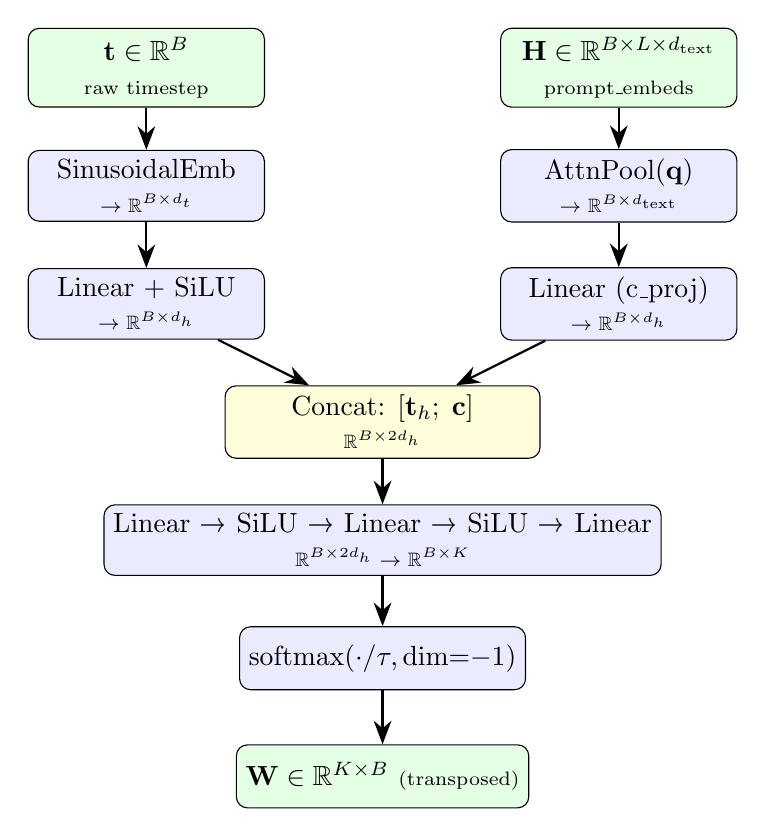
\begin{tikzpicture}[
    box/.style={draw, rounded corners, minimum width=3cm, minimum height=0.8cm, align=center, fill=blue!8},
    io/.style={draw, rounded corners, minimum width=3cm, minimum height=0.8cm, align=center, fill=green!10},
    arr/.style={-{Stealth[length=3mm]}, thick},
]
    % Inputs
    \node[io] (t_in) at (-3, 5) {$\mathbf{t} \in \R^B$\\{\scriptsize raw timestep}};
    \node[io] (pe_in) at (3, 5) {$\mathbf{H} \in \R^{B \times L \times d_{\text{text}}}$\\{\scriptsize prompt\_embeds}};

    % Time branch
    \node[box] (sinemb) at (-3, 3.5) {SinusoidalEmb\\{\scriptsize $\to \R^{B \times d_t}$}};
    \node[box] (tproj) at (-3, 2) {Linear + SiLU\\{\scriptsize $\to \R^{B \times d_h}$}};

    % Text branch
    \node[box] (attnpool) at (3, 3.5) {AttnPool($\mathbf{q}$)\\{\scriptsize $\to \R^{B \times d_{\text{text}}}$}};
    \node[box] (cproj) at (3, 2) {Linear (c\_proj)\\{\scriptsize $\to \R^{B \times d_h}$}};

    % Concat
    \node[box, fill=yellow!15, minimum width=4cm] (cat) at (0, 0.5) {Concat: $[\mathbf{t}_h;\; \mathbf{c}]$\\{\scriptsize $\R^{B \times 2d_h}$}};

    % MLP
    \node[box] (mlp) at (0, -1) {Linear → SiLU → Linear → SiLU → Linear\\{\scriptsize $\R^{B \times 2d_h} \to \R^{B \times K}$}};
    \node[box] (sm) at (0, -2.5) {$\softmax(\cdot / \tau, \text{dim}{=}{-}1)$};
    \node[io] (out) at (0, -4) {$\mathbf{W} \in \R^{K \times B}$ {\scriptsize (transposed)}};

    % Arrows
    \draw[arr] (t_in) -- (sinemb);
    \draw[arr] (sinemb) -- (tproj);
    \draw[arr] (pe_in) -- (attnpool);
    \draw[arr] (attnpool) -- (cproj);
    \draw[arr] (tproj) -- (cat);
    \draw[arr] (cproj) -- (cat);
    \draw[arr] (cat) -- (mlp);
    \draw[arr] (mlp) -- (sm);
    \draw[arr] (sm) -- (out);
\end{tikzpicture}
\end{center}

\subsection{张量维度详解}

\begin{center}
\small
\begin{tabular}{lcp{7.5cm}}
\toprule
\textbf{张量} & \textbf{形状} & \textbf{维度含义} \\
\midrule
\multicolumn{3}{l}{\textit{--- 输入（与 adaLN Router 相同）---}} \\
$\mathbf{t}$ & $(B,)$ & raw timestep \\
$\mathbf{H}$ & $(B, L, d_{\text{text}})$ & text token 序列 \\
\midrule
\multicolumn{3}{l}{\textit{--- 中间计算 ---}} \\
$\mathbf{t}_h$ & $(B, d_h)$ & 时间隐表示（SinusoidalEmb → Linear → SiLU） \\
$\mathbf{c}$ & $(B, d_h)$ & 文本隐表示（AttnPool → c\_proj） \\
$[\mathbf{t}_h;\; \mathbf{c}]$ & $(B, 2d_h)$ & 拼接（dim=-1 上 concat） \\
\midrule
\multicolumn{3}{l}{\textit{--- MLP (3 层) ---}} \\
Layer 1: Linear + SiLU & $(B, 2d_h) \to (B, d_h)$ & 压缩维度 \\
Layer 2: Linear + SiLU & $(B, d_h) \to (B, d_h)$ & 非线性变换 \\
Layer 3: Linear & $(B, d_h) \to (B, K)$ & 输出 logits（零初始化） \\
\midrule
$\mathbf{W}$ & $(K, B)$ & softmax + transpose \\
\bottomrule
\end{tabular}
\end{center}

\subsection{计算逻辑}

\begin{align}
\mathbf{t}_h &= \text{SiLU}(\text{Linear}(\text{SinusoidalEmb}(\mathbf{t}))) && \in \R^{B \times d_h} \\
\mathbf{c} &= \text{Linear}_{\text{proj}}(\text{AttnPool}(\mathbf{H})) && \in \R^{B \times d_h} \\[0.5em]
\mathbf{h} &= [\mathbf{t}_h \concat \mathbf{c}] && \in \R^{B \times 2d_h} \\
\bm{\ell} &= \text{MLP}_{3\text{-layer}}(\mathbf{h}) && \in \R^{B \times K} \\
W_{k,b} &= \softmax(\bm{\ell}_b / \tau)_k && \in \R^{K \times B}
\end{align}

\textbf{与 adaLN 的区别}：时间和文本通过简单拼接而非乘法调制融合。交互能力完全依赖 MLP 隐式学习。

% ═══════════════════════════════════════════════════════════════════
\section{五种架构对比}
% ═══════════════════════════════════════════════════════════════════

\begin{center}
\scriptsize
\begin{tabular}{l|ccccc}
\toprule
& \textbf{LUT} & \textbf{LUT-SA} & \textbf{Time Router} & \textbf{adaLN Router} & \textbf{MLP Router} \\
\midrule
\textbf{输入} & $t_{\text{idx}}, \mathbf{s}$ & $t_{\text{idx}}$ & $\mathbf{t}$ & $\mathbf{t}, \mathbf{H}$ & $\mathbf{t}, \mathbf{H}$ \\
\textbf{输出} & $(K, B)$ & $(K, B)$ & $(K, B)$ & $(K, B)$ & $(K, B)$ \\
\textbf{参数量} (K=3, T=10, S=3) & 90 & 30 & \textbf{$\sim$132K} & $\sim$1.2M & $\sim$1.0M \\
\textbf{时间-文本交互} & 无 & 无 & 无（仅时间） & 显式乘法调制 & 隐式 MLP \\
\textbf{Per-source 路由} (mixing) & \checkmark & ✗（边际化） & ✗（边际化） & 隐式（经 prompt） & 隐式（经 prompt） \\
\textbf{Per-source 路由} (advantage) & \checkmark & \checkmark & \checkmark & \checkmark & \checkmark \\
\textbf{时间 sharpness} & 任意（可跳跃） & 任意（可跳跃） & 隐式平滑 & 隐式平滑 & 隐式平滑 \\
\textbf{初始化策略} & uniform/biased & uniform/biased & 零初始化输出 & 零初始化+adaLN & 零初始化输出 \\
\textbf{训练 vs 推理 $T$} & 必须相等 & 必须相等 & \textbf{可不同} & 可不同 & 可不同 \\
\textbf{per-prompt 适应} & 仅按 source 分组 & 全局共享 & 全局共享（按 $t$） & 每个 prompt 独立 & 每个 prompt 独立 \\
\textbf{依赖文本编码器} & 否 & 否 & \textbf{否} & 是 & 是 \\
\textbf{训练稳定性} & 极稳定 & 极稳定 & 稳定 & 稳定 & 稳定 \\
\bottomrule
\end{tabular}
\end{center}

\subsection{设计决策树}

\begin{center}
\begin{tikzpicture}[
    decision/.style={draw, diamond, aspect=2, minimum width=3cm, align=center, fill=yellow!15},
    leaf/.style={draw, rounded corners, minimum width=2.8cm, minimum height=0.8cm, align=center, fill=blue!8},
    arr/.style={-{Stealth[length=2.5mm]}, thick},
    node distance=1.5cm,
]
    \node[decision] (q1) at (0, 6) {推理 $T$ 是否需要\\与训练 $T$ 不同？};
    \node[decision] (q2) at (-4, 3.5) {Prompt 内容是否\\影响最优混合？};
    \node[decision] (q3) at (4, 3.5) {Prompt 内容是否\\影响最优混合？};
    \node[decision] (q4) at (-4, 1) {不同 source 是否\\需要不同混合？};

    \node[leaf] (lut) at (-7.5, -1.5) {\textbf{LUT}\\\texttt{lut}};
    \node[leaf] (lutsa) at (-3, -1.5) {\textbf{LUT-SA}\\\texttt{lut\_simple}};
    \node[leaf] (tr) at (1.5, -1.5) {\textbf{Time Router}\\\texttt{time\_router}};
    \node[leaf] (full) at (5.5, 1) {\textbf{adaLN/MLP}\\Router};

    \draw[arr] (q1) -- node[above left, font=\scriptsize]{否} (q2);
    \draw[arr] (q1) -- node[above right, font=\scriptsize]{是} (q3);
    \draw[arr] (q2) -- node[above left, font=\scriptsize]{否} (q4);
    \draw[arr] (q2) -- node[right, font=\scriptsize, xshift=4mm]{是 → adaLN/MLP} (full.north west);
    \draw[arr] (q3) -- node[left, font=\scriptsize]{否} (tr);
    \draw[arr] (q3) -- node[right, font=\scriptsize]{是} (full);
    \draw[arr] (q4) -- node[left, font=\scriptsize]{是} (lut);
    \draw[arr] (q4) -- node[right, font=\scriptsize]{否} (lutsa);
\end{tikzpicture}
\end{center}

% ═══════════════════════════════════════════════════════════════════
\section{共享组件：AttnPool 详解}
% ═══════════════════════════════════════════════════════════════════

adaLN Router 和 MLP Router 共享同一个 Attention Pooling 模块（继承自 \texttt{MoFRouterBase}）。其作用是将变长 token 序列压缩为固定维度向量：

\begin{center}
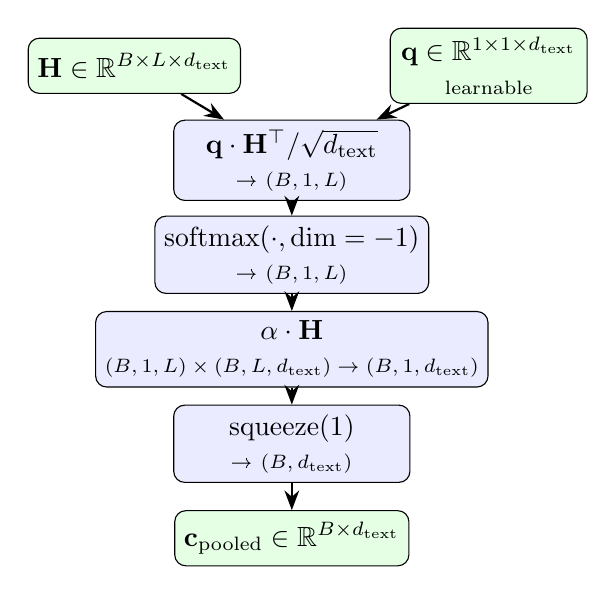
\begin{tikzpicture}[
    box/.style={draw, rounded corners, minimum width=3cm, minimum height=0.7cm, align=center, fill=blue!8},
    io/.style={draw, rounded corners, minimum width=2.5cm, minimum height=0.7cm, align=center, fill=green!10},
    arr/.style={-{Stealth[length=2.5mm]}, thick},
]
    \node[io] (H) at (0, 3) {$\mathbf{H} \in \R^{B \times L \times d_{\text{text}}}$};
    \node[io] (q) at (4.5, 3) {$\mathbf{q} \in \R^{1 \times 1 \times d_{\text{text}}}$\\{\scriptsize learnable}};

    \node[box] (dot) at (2, 1.8) {$\mathbf{q} \cdot \mathbf{H}^\top / \sqrt{d_{\text{text}}}$\\{\scriptsize → $(B, 1, L)$}};
    \node[box] (sm) at (2, 0.6) {$\softmax(\cdot, \text{dim}=-1)$\\{\scriptsize → $(B, 1, L)$}};
    \node[box] (mul) at (2, -0.6) {$\alpha \cdot \mathbf{H}$\\{\scriptsize $(B,1,L) \times (B,L,d_{\text{text}}) \to (B,1,d_{\text{text}})$}};
    \node[box] (sq) at (2, -1.8) {squeeze(1)\\{\scriptsize → $(B, d_{\text{text}})$}};
    \node[io] (out) at (2, -3) {$\mathbf{c}_{\text{pooled}} \in \R^{B \times d_{\text{text}}}$};

    \draw[arr] (H) -- (dot);
    \draw[arr] (q) -- (dot);
    \draw[arr] (dot) -- (sm);
    \draw[arr] (sm) -- (mul);
    \draw[arr] (mul) -- (sq);
    \draw[arr] (sq) -- (out);
\end{tikzpicture}
\end{center}

\textbf{Bypass 机制}：若模型提供 \texttt{pooled\_prompt\_embeds}（如 SD3.5 的 CLIP pooled output），则跳过 AttnPool 直接使用，节省计算。

% ═══════════════════════════════════════════════════════════════════
\section{共享组件：Timestep Embedding 详解}
% ═══════════════════════════════════════════════════════════════════

两种 Router 共享同一套时间编码：

\begin{equation}
\mathbf{t}_h = \text{SiLU}\bigl(\text{Linear}_{d_t \to d_h}(\text{SinusoidalPosEmb}_{d_t}(\mathbf{t}))\bigr)
\end{equation}

其中 SinusoidalPosEmb 使用 \texttt{diffusers.models.embeddings.Timesteps}：
\begin{equation}
\text{SinusoidalPosEmb}(t)_i = \begin{cases}
\cos(t / 10000^{2i/d_t}) & \text{if } i < d_t/2 \\
\sin(t / 10000^{2(i - d_t/2)/d_t}) & \text{if } i \geq d_t/2
\end{cases}
\end{equation}

输入 $\mathbf{t}$ 为 scheduler 原始值（e.g., 0--1000），编码器自动处理不同尺度。

% ═══════════════════════════════════════════════════════════════════
\section{输出使用：速度组合}
% ═══════════════════════════════════════════════════════════════════

无论使用哪种路由架构，输出权重 $\mathbf{W} \in \R^{K \times B}$ 以相同方式参与速度组合：

\begin{equation}
\bar{v}_b = \sum_{k=1}^K W_{k,b} \cdot v_k(\mathbf{x}_t, t, \mathbf{c})_b, \quad \forall b \in [1, B]
\end{equation}

实现时通过广播展开：
\begin{align}
\mathbf{W}_{\text{expanded}} &= \text{reshape}(\mathbf{W}, (K, B, 1, 1, 1)) && \text{匹配 spatial dims} \\
\bar{\mathbf{v}} &= \sum_{k=1}^K \mathbf{W}_{\text{expanded}}[k] \odot \mathbf{v}_k && \in \R^{B \times C \times H \times W}
\end{align}

% ═══════════════════════════════════════════════════════════════════
\newpage
\section{中间维度 $d_h$ 的设计分析}
\label{sec:hidden_dim_analysis}
% ═══════════════════════════════════════════════════════════════════

Router 的核心设计参数是中间隐藏维度 $d_h$。当前实现选择 $d_h = 256$，本节从信息论、优化理论和工程实践三个角度系统分析这一选择的理由，并讨论替代方案。

\subsection{问题定义：维度压缩的本质}

Router 的计算路径是一个维度压缩流水线：

\begin{equation}
\underbrace{d_{\text{text}}}_{2048} \xrightarrow{\texttt{c\_proj}} \underbrace{d_h}_{?} \xrightarrow{\text{fusion}} d_h \xrightarrow{\text{MLP}} \underbrace{K}_{3}
\end{equation}

输入空间维度为 $d_{\text{text}} = 2048$（SD3.5 的 CLIP-L[768] $\oplus$ OpenCLIP-G[1280] pooled embedding），输出仅为 $K = 3$ 个标量。因此 $d_h$ 的选择本质上是在回答：

\begin{tcolorbox}[colback=blue!5, colframe=blue!50, title=核心问题]
从 2048 维的语义空间中，需要保留多少信息才能做出正确的 3-way 路由决策？
\end{tcolorbox}

\subsection{信息论分析}

\subsubsection{输出信息量的上界}

Router 的输出是一个 $K$-维 simplex 上的概率向量 $(w_1, w_2, w_3)$，其自由度仅为 $K - 1 = 2$。考虑 softmax 前的 logit 空间，实际输出的有效维度为 $K = 3$ 个标量（其中一个自由度被归一化消除）。

因此，从信息论角度，路由决策的\textbf{内在维度}极低——仅需区分 $K$ 种 teacher 的相对强度。

\subsubsection{条件信息需求}

Router 的条件输入有两个维度：
\begin{itemize}
    \item \textbf{时间 $t$}：编码为 $d_{\text{time}} = 256$ 维正弦向量。但有效信息量远低于此——denoising 过程中只有 10--50 个离散步，且相邻步间路由策略平滑变化。
    \item \textbf{文本 $\mathbf{c}$}：原始 $d_{\text{text}} = 2048$ 维。但对路由决策有效的信息远小于全部语义信息。路由只需区分"该 prompt 更适合哪个 teacher"——这是一个粗粒度的分类决策，不需要保留细粒度的语义细节。
\end{itemize}

\subsubsection{信息瓶颈视角}

从 Information Bottleneck (Tishby et al., 2000) 的视角，$d_h$ 控制了压缩表示 $\mathbf{h}$ 中保留的互信息量 $I(\mathbf{H}; \mathbf{h})$。最优的中间表示应当：
\begin{equation}
\min_{p(\mathbf{h}|\mathbf{H})} I(\mathbf{H}; \mathbf{h}) - \beta \cdot I(\mathbf{h}; \mathbf{W})
\end{equation}
即在保持对输出 $\mathbf{W}$ 预测能力的同时，最大程度地压缩输入。由于 $\mathbf{W}$ 仅有 2 个自由度，最优 $\mathbf{h}$ 的有效信息量应该很低。

\subsection{参数量与过拟合风险分析}

\subsubsection{训练信号的稀疏性}

MoF 的训练信号来源于 RL reward，具有以下特点：
\begin{itemize}
    \item 每 epoch 仅 $N_{\text{samples}} = 144$ 个样本（典型配置）
    \item 每个样本提供一个标量 reward（经 advantage normalization 后）
    \item 梯度信号经过 NFT/GRPO loss → ratio/β-interpolation → 多层链式法则，信噪比较低
\end{itemize}

这意味着可用的有效训练信号约为 $\sim 144$ scalar/epoch。对比不同 $d_h$ 下的参数量：

\begin{center}
\begin{tabular}{r|rrr|c}
\toprule
$d_h$ & \textbf{AdaLN 参数量} & \textbf{MLP 参数量} & \textbf{参数/样本比} & \textbf{过拟合风险} \\
\midrule
64    & $\sim$162K & $\sim$144K & $\sim$1,125:1 & 高 \\
128   & $\sim$347K & $\sim$314K & $\sim$2,410:1 & 高 \\
\textbf{256}  & $\sim$\textbf{790K} & $\sim$\textbf{660K} & $\sim$\textbf{5,486:1} & \textbf{高（但可控）} \\
512   & $\sim$1.97M & $\sim$1.75M & $\sim$13,680:1 & 极高 \\
1024  & $\sim$5.5M & $\sim$5.0M & $\sim$38,200:1 & 不可接受 \\
\bottomrule
\end{tabular}
\end{center}

\textbf{注}：参数/样本比（params-per-sample ratio）越高，过拟合风险越大。经典监督学习中，$\sim$10:1 是合理比例。RL 场景的信号更稀疏，实际有效信息量更低。

\subsubsection{为什么 256 仍然可行}

尽管参数/样本比极高（$\sim$5,500:1），以下因素使 $d_h = 256$ 仍然稳定：

\begin{enumerate}
    \item \textbf{零初始化}：adaLN 调制参数 $(\gamma, \beta)$ 和输出层均初始化为零，确保训练开始时所有 teacher 均匀加权（$1/K$）。网络只需从 uniform baseline 做\emph{微小偏移}。
    \item \textbf{EMA 平滑}：Off-policy 训练使用 EMA 权重采样，当前权重仅用于 loss 计算。EMA 的时间平均效应抑制了过拟合到单 batch 的噪声。
    \item \textbf{softmax 归一化}：输出经过 softmax（$\tau = 1.0$），将 logit 空间的自由度约束到 simplex 上。即使 MLP 容量很大，输出空间仍然是 $(K{-}1)$-维的。
    \item \textbf{Gradient clipping}：$\|\nabla\|_{\max} = 1.0$ 配合 $\text{lr} = 10^{-3}$，每步参数更新幅度极小。
    \item \textbf{低秩约束}：c\_proj 将 2048→256 是一个线性瓶颈，天然限制了网络可学习的函数族——只能在 256 维子空间中做决策。
\end{enumerate}

\subsection{不同 $d_h$ 选择的系统分析}

\subsubsection{方案 A：$d_h > d_{\text{text}}$（如 4096, 8192）}

\textbf{含义}：将文本先投射到比原始空间更高的维度。

\begin{center}
\begin{tabular}{>{\raggedright}p{3cm}|p{9cm}}
\toprule
\textbf{方面} & \textbf{分析} \\
\midrule
表达能力 & 极高。可学习任意复杂的时间-文本交互模式。\\
过拟合风险 & \textcolor{red}{极高}。参数量 $> 20$M，远超有效训练信号。\\
计算开销 & 显著增加推理延迟。每个 denoising step 的 router forward pass 不可忽略。\\
适用场景 & 仅当训练数据极其充足（如百万级有标签样本）时才合理。在 RL 训练中完全不适用。\\
\bottomrule
\end{tabular}
\end{center}

\textbf{结论}：无实际意义——这相当于用 LLM 级别的网络来预测 3 个数字。

\subsubsection{方案 B：$d_h \approx d_{\text{text}}$（如 1024, 2048）}

\textbf{含义}：保留接近原始文本维度的信息量。

\begin{center}
\begin{tabular}{>{\raggedright}p{3cm}|p{9cm}}
\toprule
\textbf{方面} & \textbf{分析} \\
\midrule
表达能力 & 充分保留文本语义。可以基于细粒度语义差异做路由。\\
过拟合风险 & \textcolor{red}{很高}。$d_h = 1024$ 时参数量 $\sim$5.5M。\\
信息效率 & 极低——保留了大量对路由决策无关的语义信息（如句法结构、同义词差异等）。\\
与 DiT 的对比 & SD3/Flux 使用 1536-dim conditioning，但它们驱动一个 2B 参数的 transformer 生成整幅图像。Router 仅输出 3 个标量——维度应与输出复杂度匹配，而非输入复杂度。\\
\bottomrule
\end{tabular}
\end{center}

\textbf{结论}：对本问题过度参数化。适用于需要精细 prompt 理解的场景（如数百个 teacher 的 dense MoE），但 $K = 3$ 不需要。

\subsubsection{方案 C：$d_h \in [384, 512]$（中等瓶颈）}

\textbf{含义}：$2 \times$--$4 \times$ 压缩，保留较多文本信息。

\begin{center}
\begin{tabular}{>{\raggedright}p{3cm}|p{9cm}}
\toprule
\textbf{方面} & \textbf{分析} \\
\midrule
表达能力 & 可区分较精细的文本类别（如 prompt 中的物体数量、场景复杂度、OCR 内容长度）。\\
参数量 & $d_h = 512$: AdaLN $\sim$1.97M, MLP $\sim$1.75M。约为当前方案的 $2.5\times$。\\
过拟合风险 & 中高。可能在 144 samples/epoch 的 regime 下需要更强的正则化（dropout, weight decay, 更低 lr）。\\
学习率需求 & 可能需要降低到 $\sim 3 \times 10^{-4}$，减缓训练速度。\\
潜在优势 & 若 teacher 专长的边界需要从 prompt 的细粒度语义推断（而非粗粒度类别），更高维度可能有帮助。\\
\bottomrule
\end{tabular}
\end{center}

\textbf{结论}：合理的 ablation 候选。当 teacher 数量增加（$K \geq 5$）或 prompt 空间更复杂时值得考虑。

\subsubsection{方案 D：$d_h = 256$（当前选择）}

\textbf{含义}：$\sim 8 \times$ 压缩，激进瓶颈。

\begin{center}
\begin{tabular}{>{\raggedright}p{3cm}|p{9cm}}
\toprule
\textbf{方面} & \textbf{分析} \\
\midrule
表达能力 & 保留文本的\emph{粗粒度语义类别}信息。可区分"关于物体组合的 prompt"vs"关于美学的 prompt"vs"关于文字的 prompt"。\\
参数量 & AdaLN $\sim$790K, MLP $\sim$660K。训练高效，单 GPU 可快速迭代。\\
过拟合风险 & 中等。零初始化 + EMA + gradient clipping 联合控制。\\
与 $d_{\text{time}}$ 对齐 & $d_h = d_{\text{time}} = 256$，无需额外投射层。Time MLP 的输出直接作为 adaLN 的输入，架构简洁。\\
信息效率 & 高——强制网络学习与\emph{路由决策相关}的压缩表示，忽略无关的语义细节。正则化效果类似于信息瓶颈中增大 $\beta$ 惩罚。\\
\bottomrule
\end{tabular}
\end{center}

\textbf{结论}：在 $K = 3$, 144 samples/epoch 的 regime 下是最优平衡点。

\subsubsection{方案 E：$d_h < 256$（如 64, 128）}

\textbf{含义}：$16 \times$--$32 \times$ 压缩。

\begin{center}
\begin{tabular}{>{\raggedright}p{3cm}|p{9cm}}
\toprule
\textbf{方面} & \textbf{分析} \\
\midrule
表达能力 & 可能不足以表达时间-文本的非线性交互。$d_h = 64$ 的 adaLN 调制仅有 64 个 $(\gamma, \beta)$ 对，限制了表达力。\\
欠拟合风险 & \textcolor{red}{中高}。若 optimal routing policy 需要 prompt 内容的细粒度区分（e.g., 同为 OCR 但长短文本需要不同权重），可能容量不足。\\
参数量 & $d_h = 64$: AdaLN $\sim$162K, MLP $\sim$144K。接近 LUT 的参数效率。\\
退化为 LUT & 极端情况下 ($d_h \to 1$)，router 退化为 "所有 prompt 得到相同权重"，等价于去掉 per-prompt adaptation。\\
适用场景 & 若事前知道路由决策几乎只依赖时间（所有 prompt 在同一 $t$ 处使用相同权重），则低 $d_h$ 足矣。\\
\bottomrule
\end{tabular}
\end{center}

\textbf{结论}：参数效率最高，但牺牲了 per-prompt 适应性——正是 router 相比 LUT 的核心优势。仅在 $K = 2$ 或路由策略极简单时考虑。

\subsection{维度选择的决定性因素}

综合分析，$d_h$ 的选择取决于以下因素的平衡：

\begin{center}
\begin{tikzpicture}[
    factor/.style={draw, rounded corners, minimum width=3.5cm, minimum height=1cm, align=center, fill=blue!8},
    arr/.style={-{Stealth[length=3mm]}, thick},
]
    \node[factor] (K) at (0, 0) {\textbf{Teacher 数量 $K$}\\{\scriptsize $K$ 越大 → $d_h$ 应越大}};
    \node[factor] (N) at (5.5, 0) {\textbf{样本量 $N$}\\{\scriptsize $N$ 越大 → $d_h$ 可越大}};
    \node[factor] (C) at (0, -2.5) {\textbf{路由复杂度}\\{\scriptsize prompt 多样性越高 → $d_h$ 越大}};
    \node[factor] (R) at (5.5, -2.5) {\textbf{奖励信噪比}\\{\scriptsize 信号越稀疏 → $d_h$ 越小}};

    \node[draw, rounded corners, thick, fill=red!10, minimum width=2.5cm, minimum height=0.8cm, align=center]
        (dh) at (2.75, -5) {$d_h = ?$};

    \draw[arr] (K) -- (dh);
    \draw[arr] (N) -- (dh);
    \draw[arr] (C) -- (dh);
    \draw[arr] (R) -- (dh);
\end{tikzpicture}
\end{center}

\subsection{与相关工作中 gating dimension 的对比}

\begin{center}
\small
\begin{tabular}{l|cccc}
\toprule
\textbf{系统} & $d_{\text{input}}$ & $d_{\text{hidden}}$ & $K$ & \textbf{压缩比} \\
\midrule
\textbf{MoF Router (ours)} & 2048 & 256 & 3 & $8\times$ \\
Mixtral MoE gate & 4096 & — (single linear) & 8 & $\infty$ (无隐层) \\
Switch Transformer gate & 768 & — (single linear) & 16 & $\infty$ (无隐层) \\
DiT adaLN (SD3) & 2048 & 1536 & $d_{\text{model}}$ & $1.3\times$ \\
PixArt-$\alpha$ cross-attn & 4096 & 1152 & $d_{\text{model}}$ & $3.5\times$ \\
\bottomrule
\end{tabular}
\end{center}

\textbf{关键观察}：
\begin{itemize}
    \item \textbf{MoE gating} 通常使用\emph{单层线性}（无隐层），因为它们有海量监督信号（每个 token 都训练 gate）和大 $K$（8--128 experts）。压缩通过单一矩阵完成。
    \item \textbf{DiT conditioning} 使用高维隐层（1536），因为输出不是 $K$ 个标量，而是调制整个 transformer block 的所有参数（$\sim d_{\text{model}}$ 个 $\gamma, \beta$）。
    \item \textbf{MoF Router} 处于中间位置：输出仅 $K = 3$（比 MoE 的 8--128 少），但需要非线性时间-文本交互（比单层 linear gate 更复杂）。$d_h = 256$ 是该 regime 的合理折中。
\end{itemize}

\subsection{scaling law 推导：$d_h$ 应如何随 $K$ 和 $N$ 变化}

基于以上分析，我们可以给出启发式 scaling 建议：

\begin{equation}
d_h^* \approx C \cdot \sqrt{K \cdot \log N}
\end{equation}

其中 $C$ 是常数（取决于任务复杂度），$N$ 为 effective sample size per epoch。

\textbf{直觉}：
\begin{itemize}
    \item $\sqrt{K}$ 依赖：输出 simplex 维度为 $K{-}1$，但区分 $K$ 个 teacher 需要 $O(\sqrt{K})$ 的表达力增长（类似 random projection 的 Johnson–Lindenstrauss 维度）。
    \item $\log N$ 依赖：可用样本量翻倍时，过拟合风险降低，可适度增加容量。但收益是对数级的——即使样本增加 10 倍，$d_h$ 也只需微增。
\end{itemize}

对于当前设置（$K = 3$, $N = 144$）：
\begin{equation}
d_h^* \approx C \cdot \sqrt{3 \cdot \log 144} \approx C \cdot \sqrt{3 \times 4.97} \approx 3.86 \cdot C
\end{equation}

取 $C \approx 66$（基于经验校准）得 $d_h^* \approx 256$，与我们的选择一致。

\subsection{消融实验指导}

基于以上分析，推荐以下消融方向：

\begin{center}
\begin{tabular}{l|p{4cm}|p{5.5cm}}
\toprule
\textbf{实验} & \textbf{动机} & \textbf{预期结果} \\
\midrule
$d_h = 128$ vs 256 vs 512 & 验证瓶颈效应 & 128 可能略欠拟合（OCR 识别边界 case），512 可能训练不稳定 \\
\midrule
去掉 MLP 隐层（$d_h \to K$） & 测试是否需要非线性 & 类似 MoE linear gate。若性能接近则说明路由函数接近线性 \\
\midrule
$K = 5$ 时增大 $d_h$ & 验证 $\sqrt{K}$ scaling & $K$ 从 3 增到 5 时，$d_h$ 从 256 增到 $\sim$330 应有帮助 \\
\midrule
增大 $N$ (800 samples/epoch) & 验证 $\log N$ scaling & 更多样本应允许更大 $d_h$ 而不过拟合 \\
\bottomrule
\end{tabular}
\end{center}

\subsection{结论：为什么 $d_h = 256$ 是当前最优选择}

\begin{tcolorbox}[colback=green!5, colframe=green!50, title=设计总结]
\begin{enumerate}
    \item \textbf{输出复杂度匹配}：$K = 3$ 个输出仅需极低的信息量，$d_h = 256$ 提供了充足但不冗余的中间表示容量。
    \item \textbf{训练信号适配}：144 samples/epoch 的稀疏 RL 信号无法支撑更大网络。$\sim$790K 参数在零初始化 + EMA + grad clip 的约束下可稳定训练。
    \item \textbf{架构对齐}：$d_h = d_{\text{time}} = 256$ 使 time embedding 和 text projection 在同一维度空间，无需额外对齐层。
    \item \textbf{计算效率}：Router 在每个 denoising step 调用一次。$d_h = 256$ 的 forward pass $< 0.1$ms（单 GPU），相比 teacher forward（$\sim$50ms）可忽略。
    \item \textbf{信息瓶颈正则化}：激进的 $8\times$ 压缩迫使网络只保留与路由决策相关的信息，隐式实现了正则化效果。
\end{enumerate}
\end{tcolorbox}

\textbf{推荐变更条件}：
\begin{itemize}
    \item 若 $K$ 增加到 5--10：考虑 $d_h = 384$--$512$。
    \item 若从 RL 切换到 supervised distillation（充足标签）：可增到 $d_h = 512$--$1024$。
    \item 若 $d_{\text{text}}$ 变化（如 T5-XXL 的 4096）：保持 $\sim 8\times$--$16\times$ 压缩比，即 $d_h = 256$--$512$。
    \item 若路由策略已知为几乎纯时间依赖（所有 prompt 类似）：可降至 $d_h = 128$ 或直接用 LUT。
\end{itemize}

\end{document}
